\section{Workflow}
I designed the following workflow for the project:

\subsection{Formulation of problem statement}
The problem statement as I described will be to form a autonomous vehicle. This will include creation of dataset, neural network training, and testing that neural network in the simulator (GTA-V).

\subsection{Creating dataset}
Due to the shortage to dataset, dataset needs to be created while manually controlling the vehicle in the simulator.

\subsection{Data Preprocessing}
Some data preprocessing is needed to be convert the dataset into neural network training ready data.

\subsection{Designing Neural Network}
A neural network needs to be designed which will be inspired from the Transformer Neural Networks.

\subsection{Training Neural Network}
Using the created dataset and designed model, the neural network needs to be trined and tested from the dataset.

\subsection{Simulation in GTA-V}
Once the neural network with training reaches efficient accuracy, with the help of the neural network, the vehicle needs to be driven autonomously in the simulator.

\begin{figure}[h]
    \centering
    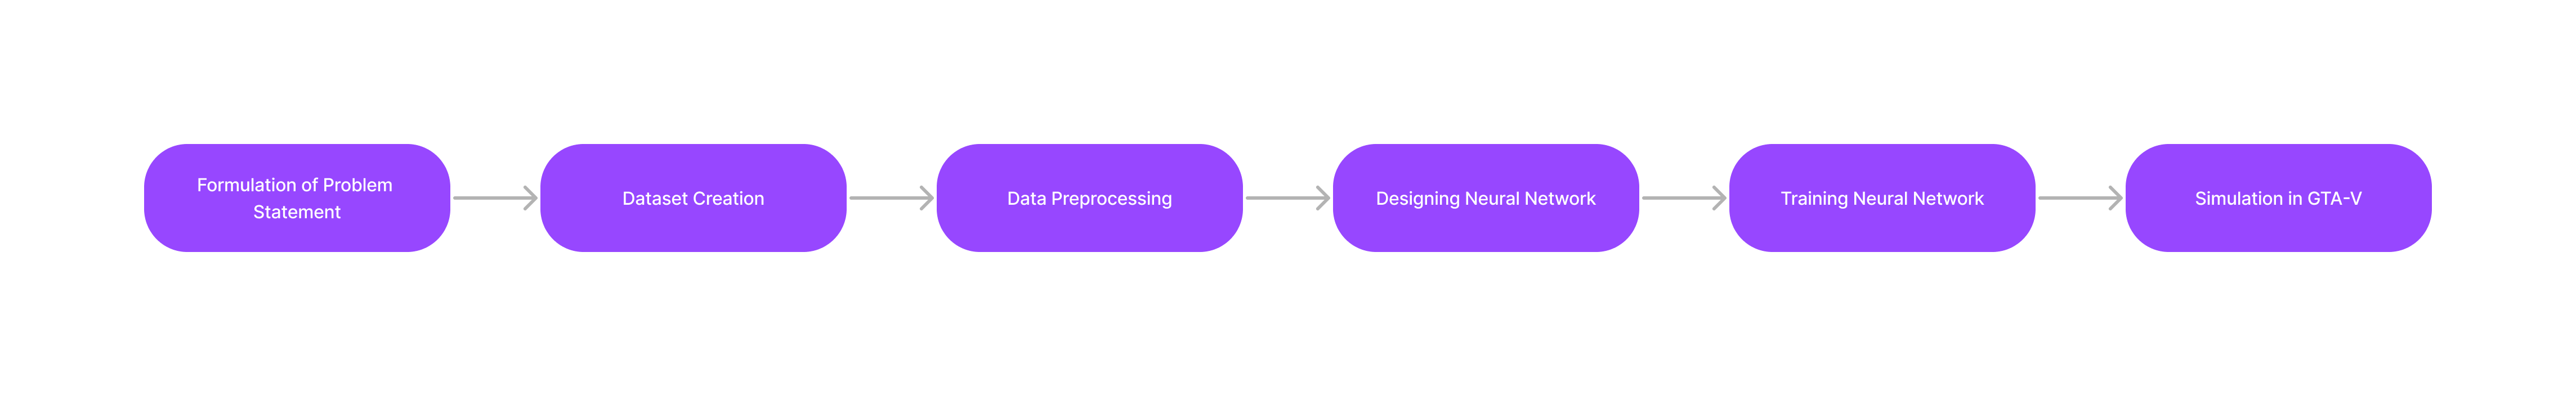
\includegraphics[width = 6in]{Ch03/workflow.png}
    \caption{Project Workflow}
    \label{figure:1}
\end{figure}
\FloatBarrier

\section{Dataset}
Since there is shortage of dataset, I have created a program to generate a dataset while a user plays the game. The data recorded consists of an image and 4 required labels.
//
A total of 10016 images and labels are recorded in the code. 

\subsection{Image}
Image of resolution 1920 X 1080 is recorded while manually controlling vehicle in the simulator. Figure 3.1 shows a image recorded image.
\begin{figure}[h]
    \centering
    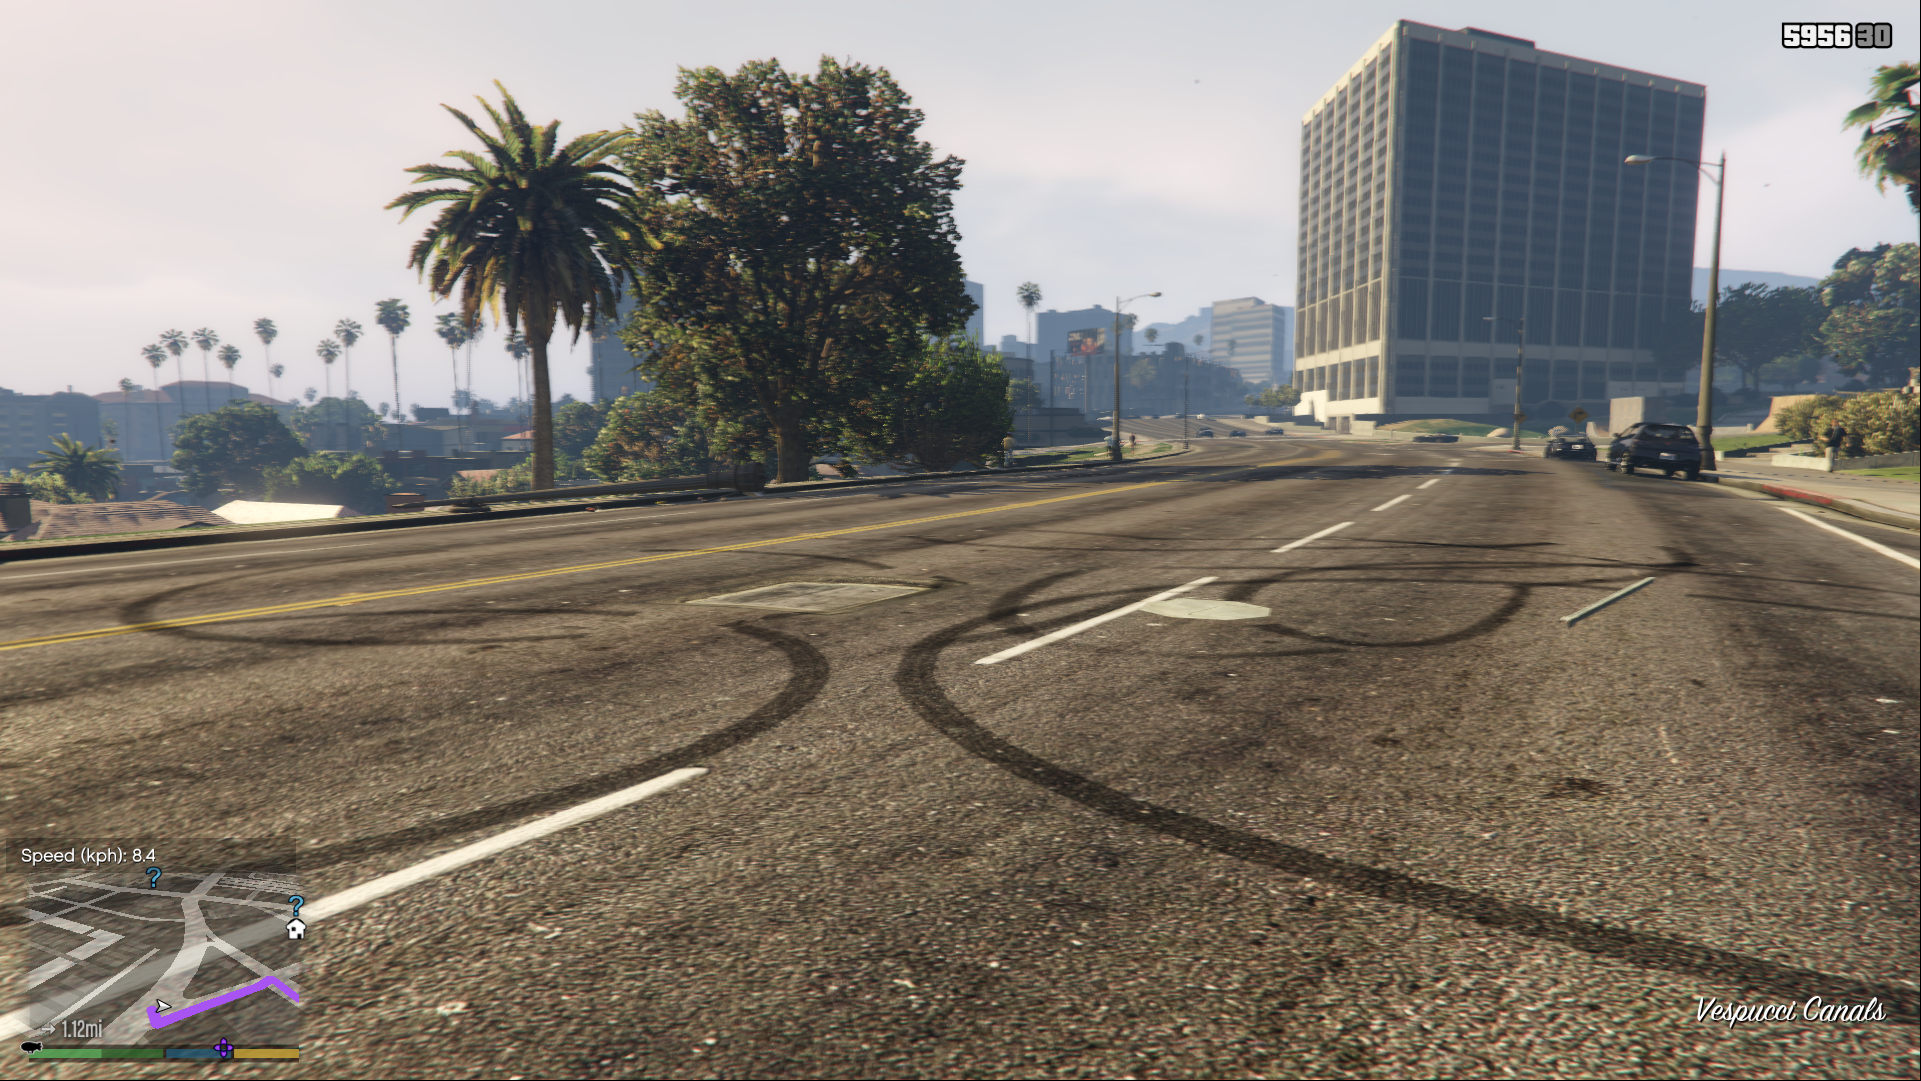
\includegraphics[width = 4in]{Ch03/0000001.png}
    \caption{Recorded Image}
    \label{figure:2}
\end{figure}
\FloatBarrier

\subsection{Labels}
The dataset comprises of four labels:
\begin{itemize}
    \item \textbf{\textit{Throttle Value}} is the value of the acceleration the car is in. Throttle value 1.0 means forward acceleration, 0.0 means backward acceleration and 0.5 means no acceleration.
    \item \textbf{\textit{Throttle Flag}} is a boolean value which states whether there is an acceleration.
    \item \textbf{\textit{Steering Value}} is the value of the steering of the car. Steering value 1.0 means left steering, 0.0 means right steering and 0.5 means no steering.
    \item \textbf{\textit{Steering Flag}} is a boolean value which states whether there is an steering.
\end{itemize}

\section{Data Preprocessing}

\subsection{Generating Navigation Map}
The Navigation System inbuilt in the game is extracted from the recorded image for coordinates (28,873) to (300,1045). Then since only the purple region is required to give the  path, it is colored white ann the rest part is colored black. Then the image is resized to 128 X 128.

\subsection{Generating Speed Map}
Using a modification in GTA-V, it is possible to have a digital speedometer which is just above the Navigation Map. From there, the speed is cropped from (125,843) to (173,869). Then the image is made binary. Then the extracted image is resized to 128 X 128.

\subsection{Resizing Image}
Since the map and speed is extracted from the original image, the region in image containing map and speed is masked to not contail it in the image. The region masked is from (20,839) to (300,1060). Then the image is resized to 256 X 256 to make the image computationally feasible for Neaural Network training. 
\\
Figure 3.2 shows the processed images, map, speed.
\begin{figure}[h]
    \centering
    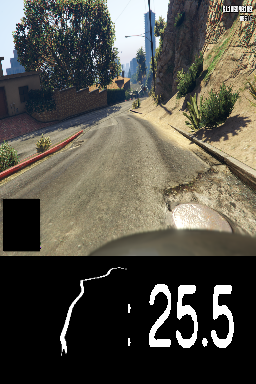
\includegraphics[width = 3in]{Ch03/final.png}
    \caption{Processed Images}
    \label{figure:3}
\end{figure}
\FloatBarrier

\subsection{Data Analysis}
Since the data has been generated recently, it has to be analysed to confirm that all attributes are in balanced. The dataset comprises of three throttle and steering values combining them forms 9 different types of labels. The following are the unique labels:
\begin{itemize}
    \item $0.0$\_$0.0$
    \item $0.0$\_$0.5$
    \item $0.0$\_$1.0$
    \item $0.5$\_$0.0$
    \item $0.5$\_$0.5$
    \item $0.5$\_$1.0$
    \item $1.0$\_$0.0$
    \item $1.0$\_$0.5$
    \item $1.0$\_$1.0$
\end{itemize}
The total number of data of each attributed has to be calculated to validate that the dataset is balanced. Figure 3.4 shows that the data is unbalanced.
\begin{figure}[h]
    \centering
    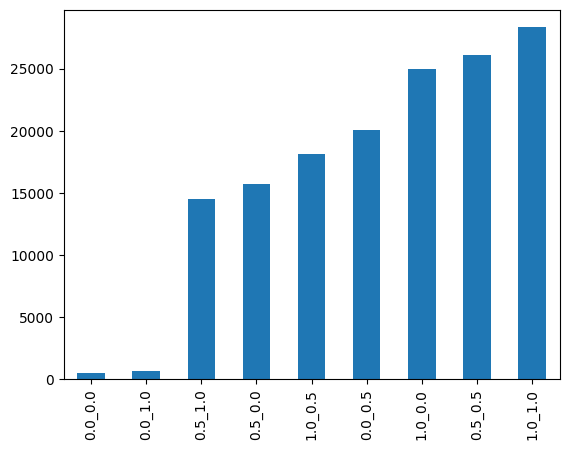
\includegraphics[width = 5in]{Ch03/unbalanced_data.png}
    \caption{Bar Graph of the Dataset Generated}
    \label{figure:4}
\end{figure}
\FloatBarrier

\subsection{Data Augmentation}
Since the data was found unbalanced, the following augmentation techniques are applied to increase the data of each labels:
\begin{itemize}
    \item Increasing/Decreasing Brightness
    \item Increasing/Decreasing Contrast
    \item Horizontal Rotation of Image
    \item Horizontal Rotation of Radar
    \item Blurring
    \item Noising
    \item Bootstrapping
\end{itemize}
Figure 3.5 shows the data after applying these techniques.
\begin{figure}[h]
    \centering
    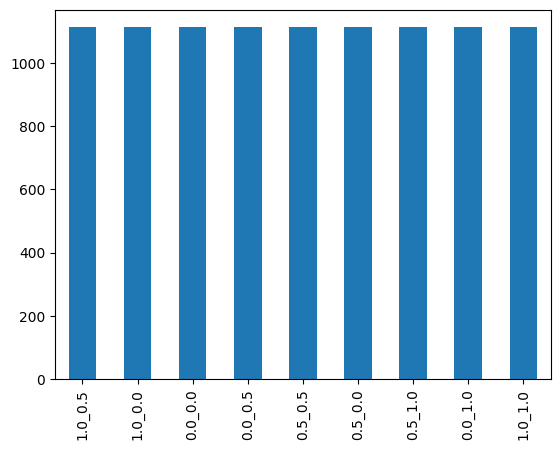
\includegraphics[width = 5in]{Ch03/balanced_data.png}
    \caption{Bar Graph of the Augmented Dataset}
    \label{figure:5}
\end{figure}
\FloatBarrier

\subsection{Collecting generate images and labels}
Then the processed images, radar and labels are pushed in an array to be saved as .npz file with images and radar saved as X and labels saved as y. A total of four such datasets are formed for training and fine-tuning. Datasets comprised of 10K, 20K, 30K, and 40K data each. The shape of:
\begin{itemize}
    \item X is [n, 2]
    \item y is [n, 4]
    \item First index of tranpose of X is (n, 256, 256, 3)
    \item Second index of tranpose of X is (n, 128, 128, 3)
\end{itemize}
where, n is the number of data in the dataset.

\section{Model Designing}
With the reference from Vision Transformer\cite{dosovitskiy2021image} and Native Transformer\cite{2017arXiv170603762V} and transformations as per the dataset, I have devised a unique transformer, named DRAN.
\\
Below is the description of the DRAN. 

\subsection{Patch Embedding}
As mentioned in the vision transformer, the image before being passed to the transformer encoder needs to be converted into patches and positional embedding needs to be added to the generated patches.
\\
For this, with the help of some online blogs, I have devised an algorithm for Patch Embedding as shown in figure 3.3.
\begin{figure}[h]
    \centering
    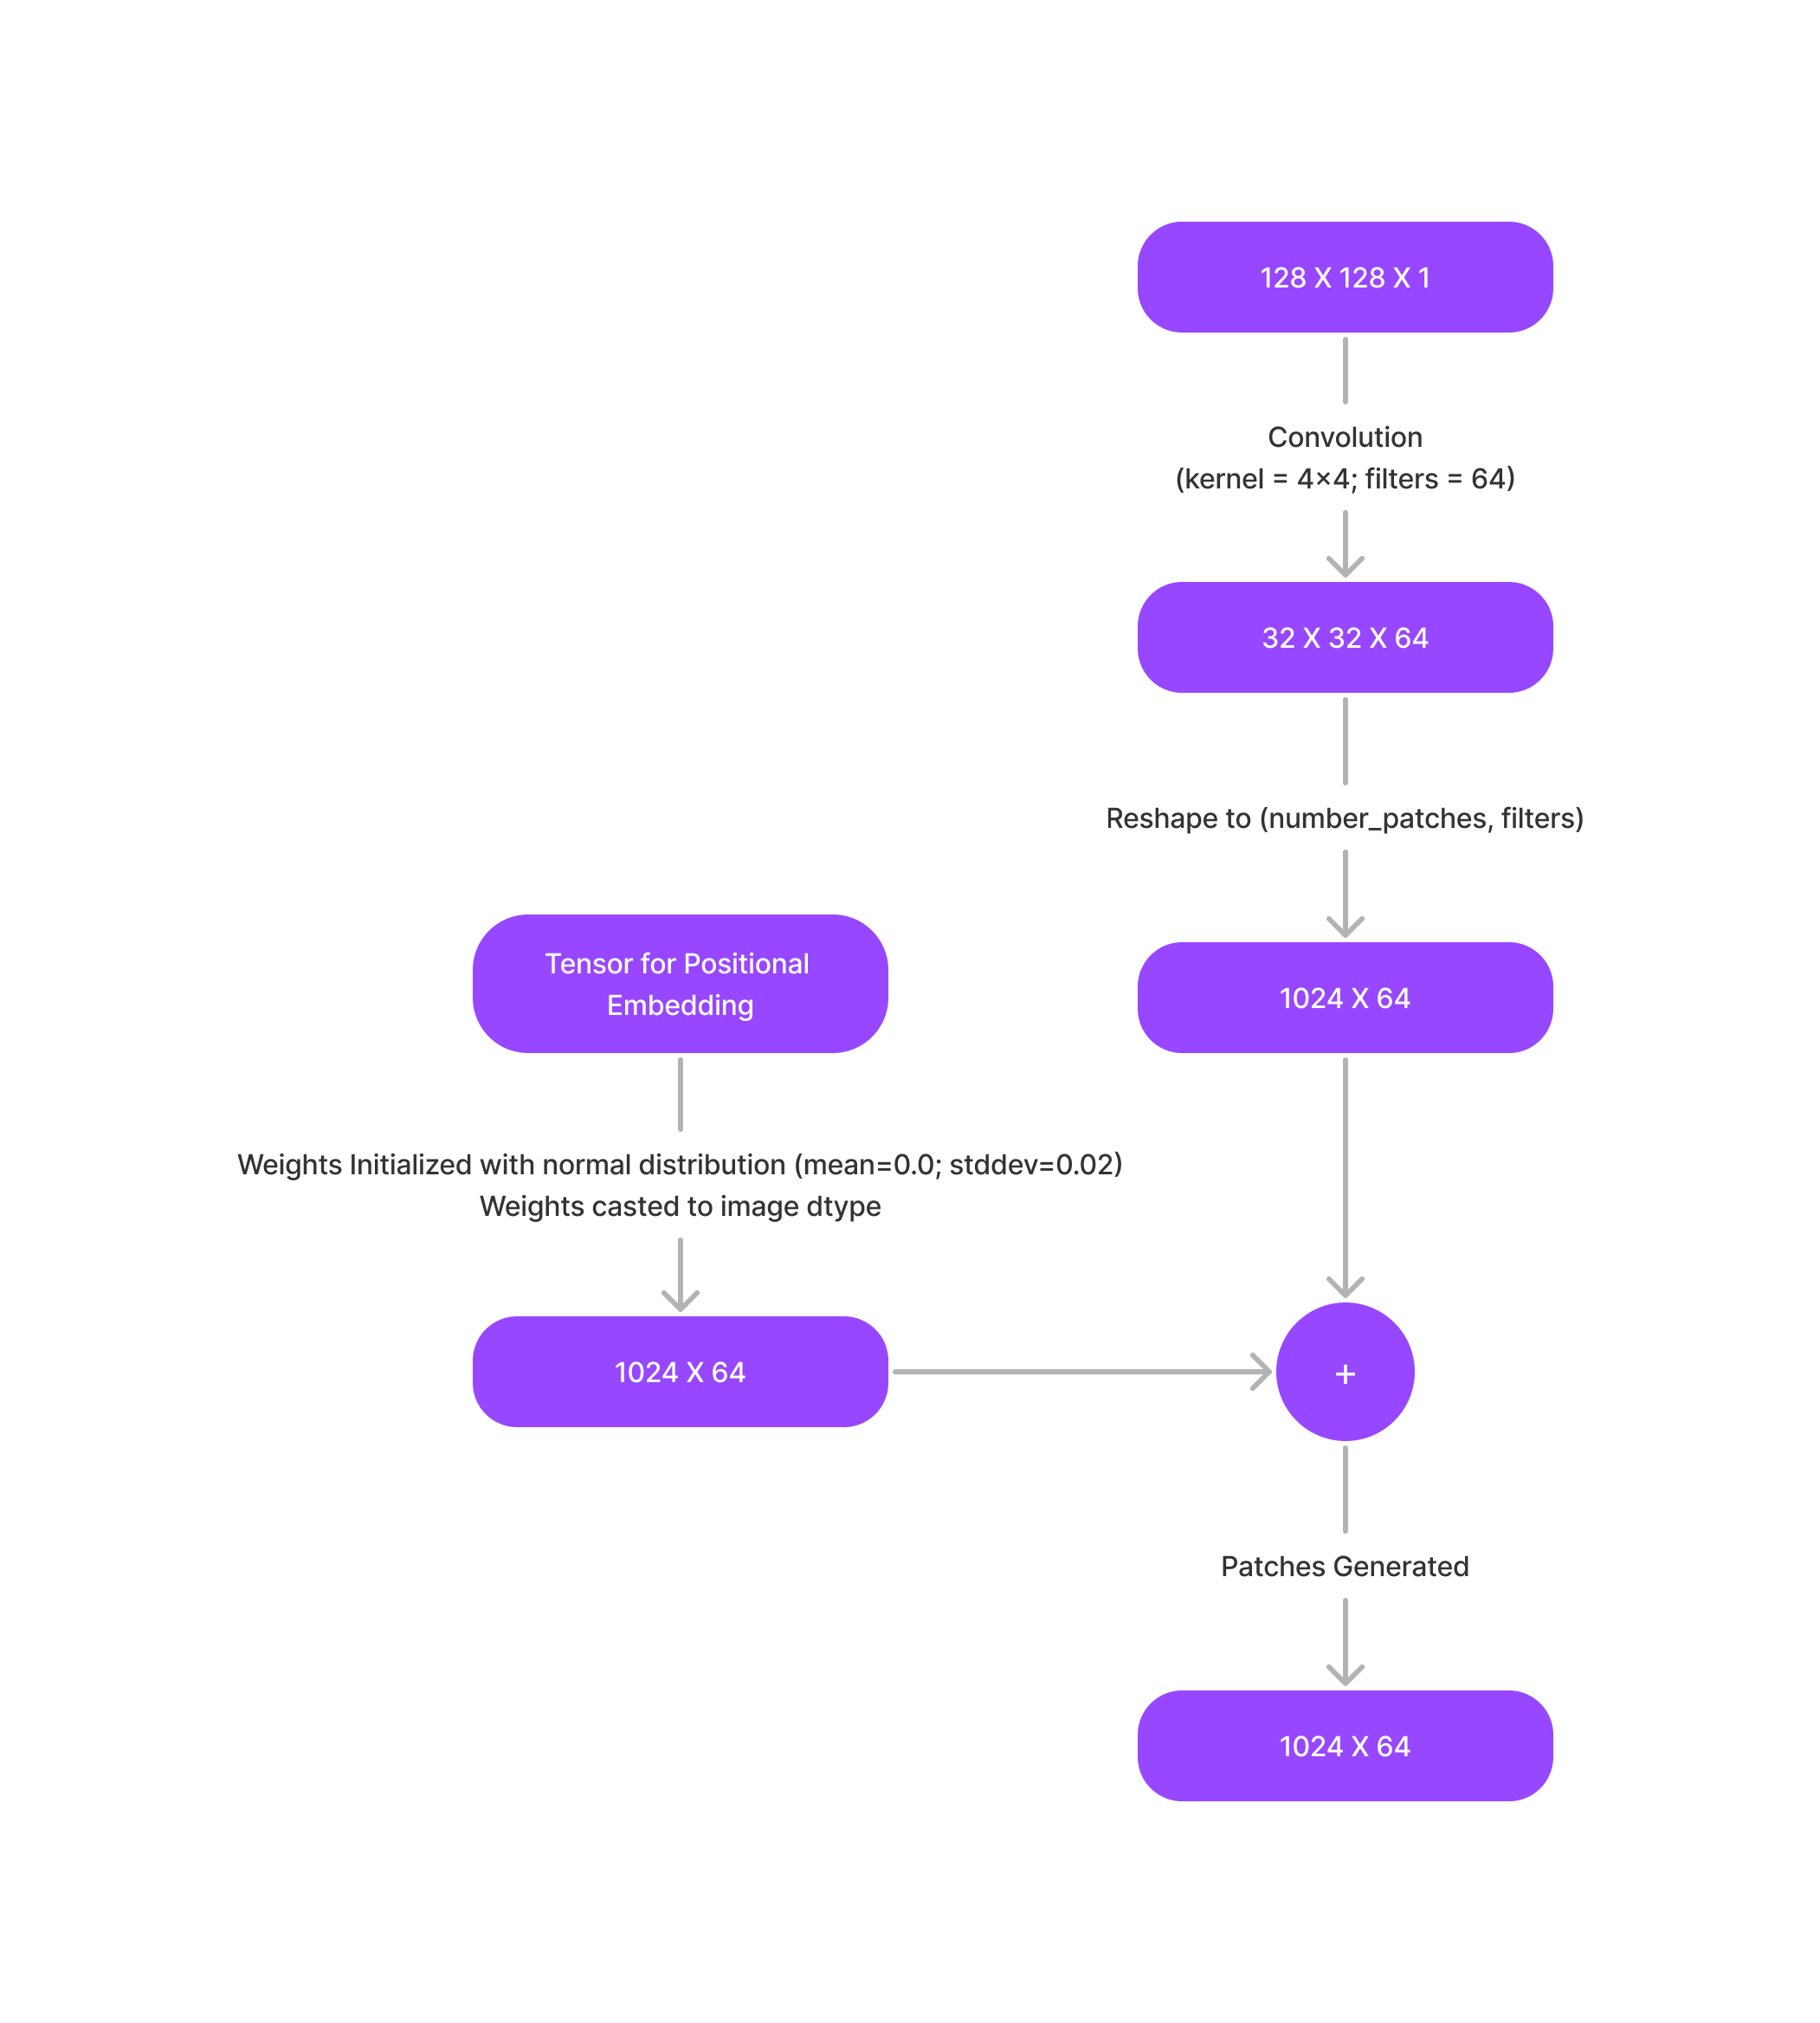
\includegraphics[width = 5in]{Ch03/patch_creation.png}
    \caption{Patch Embedding Layer}
    \label{figure:6}
\end{figure}
\FloatBarrier

\subsection{Transformer Encoder}
Encoder used in this transformer in a stack of 6 small identical units as explained in the original native transformer.

\subsection{Model Decoder}
There will be two transformer encoders in the final model so after some operations, data from two encoders will be combined and then further operations will be performed for generating output.
\\
Figure 3.4, 3.5, 3.6 represents the structure of the decoder.
\begin{figure}[h]
    \centering
    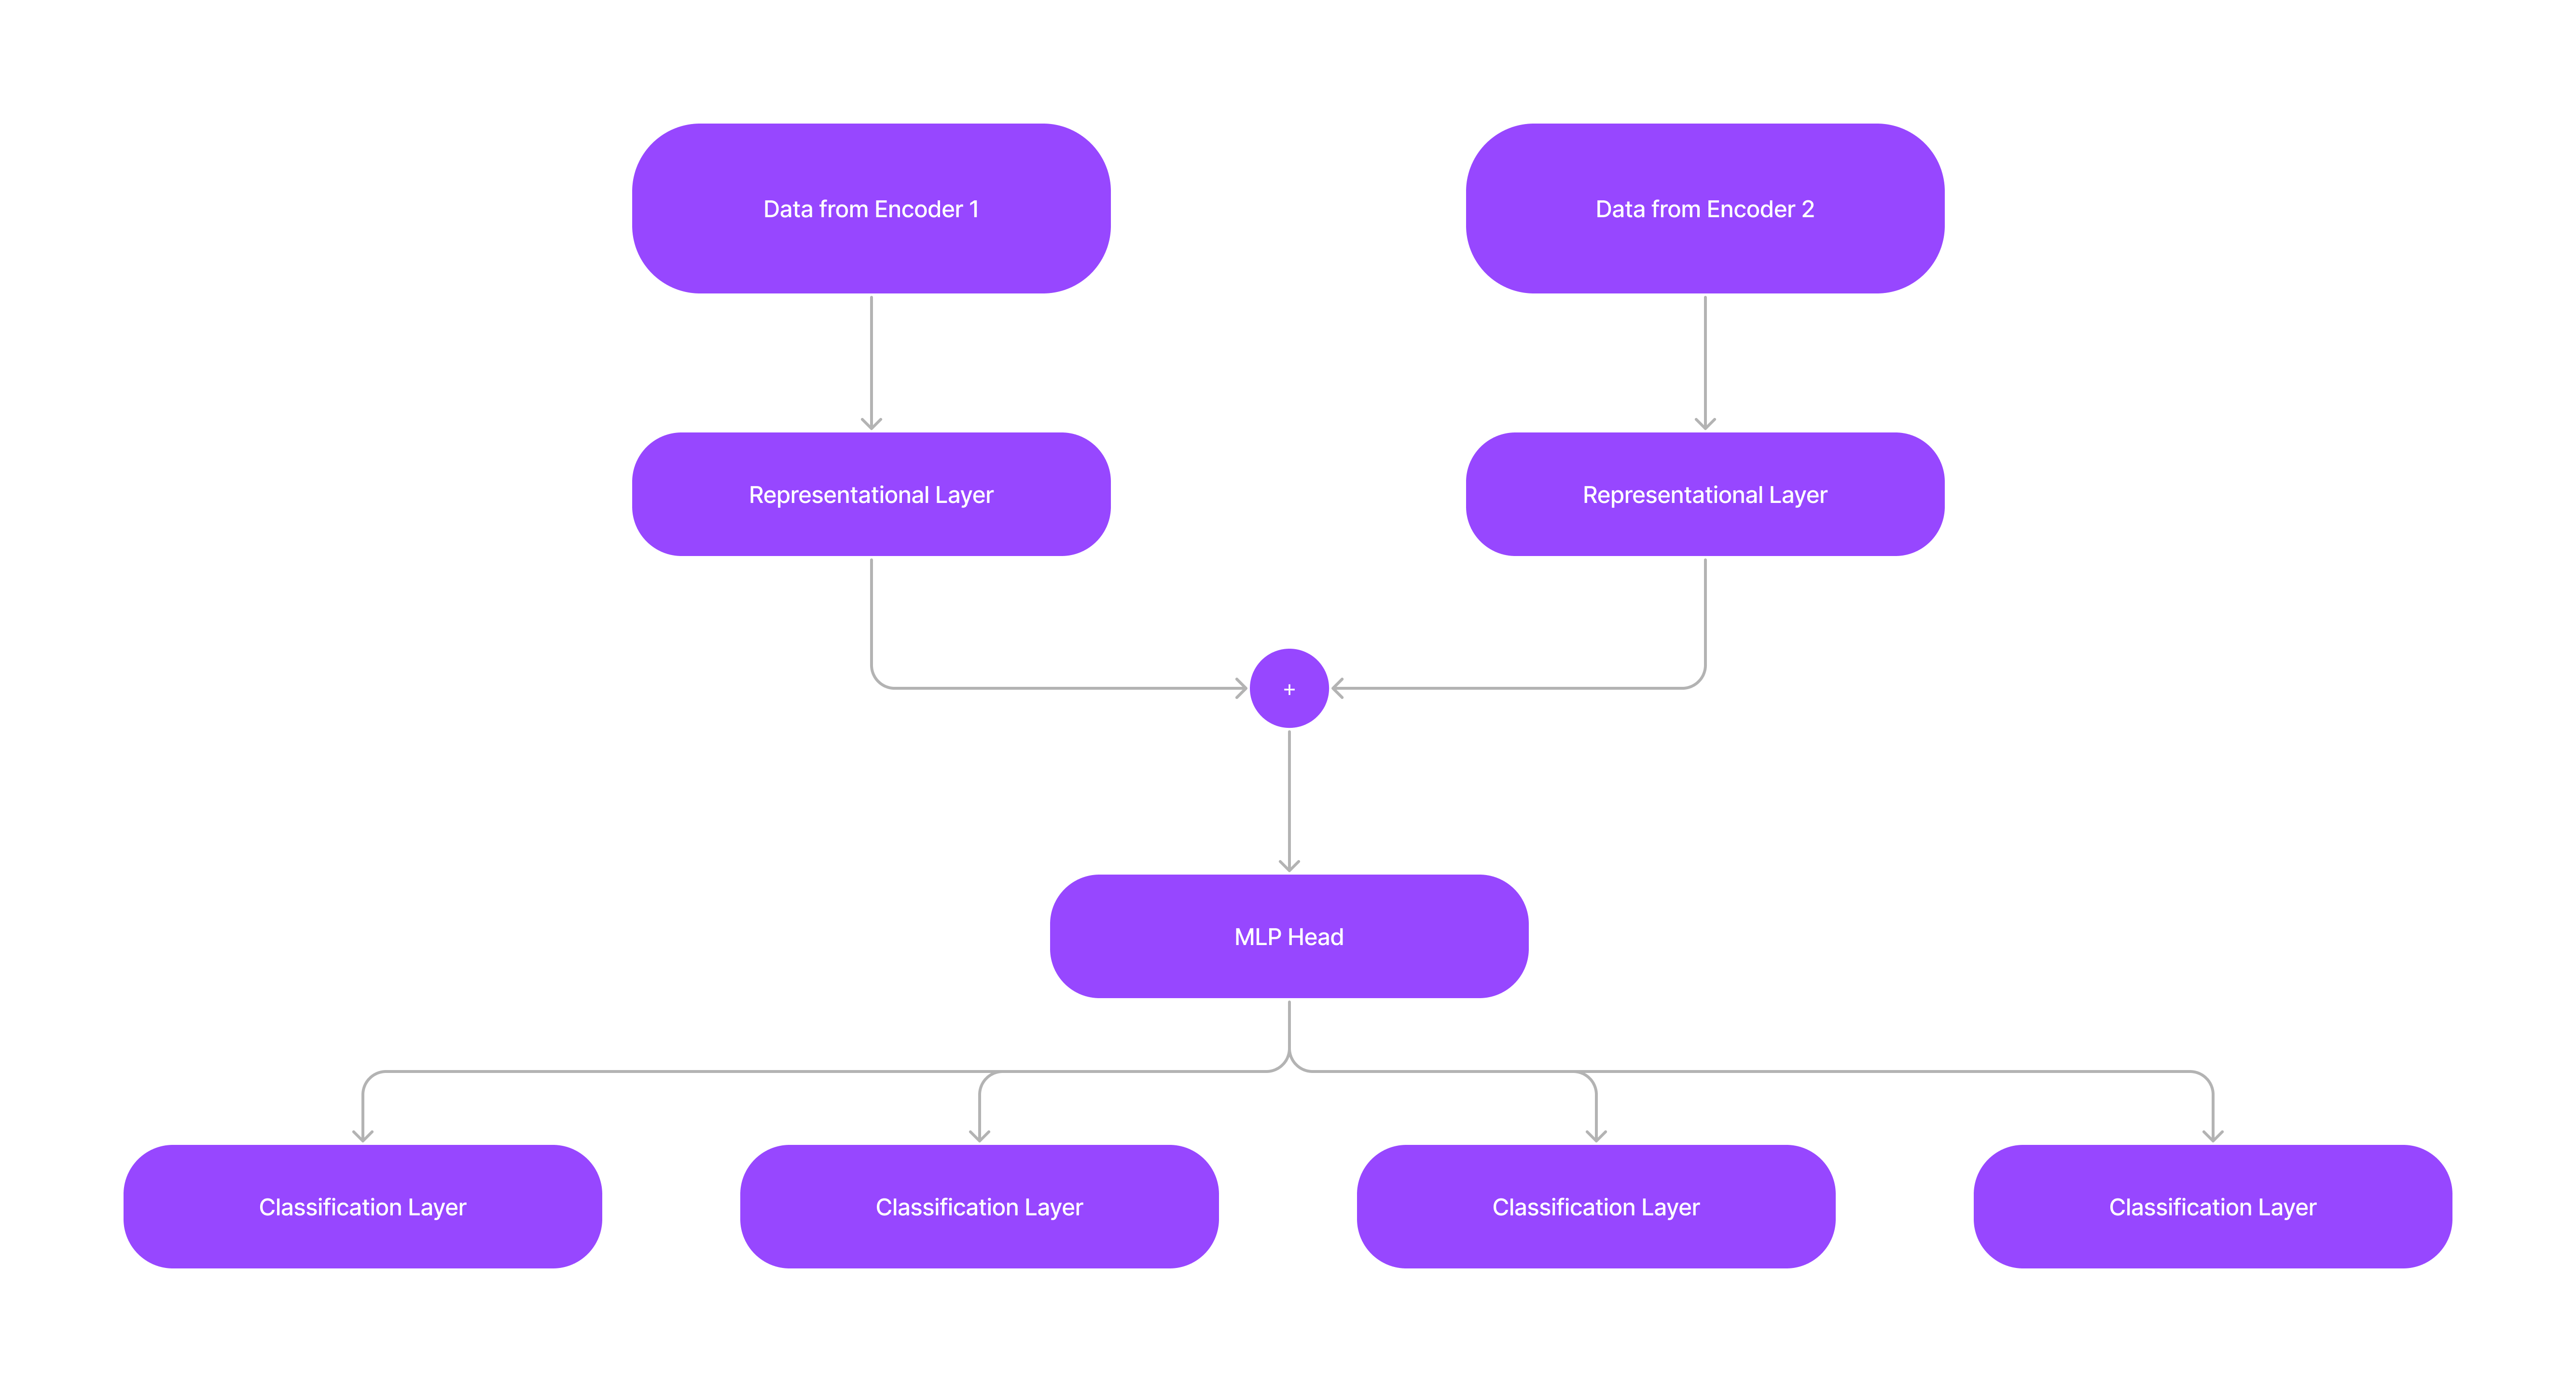
\includegraphics[width = 5in]{Ch03/model_decoder.png}
    \caption{DRAN Decoder}
    \label{figure:7}
\end{figure}
\begin{figure}[h]
    \centering
    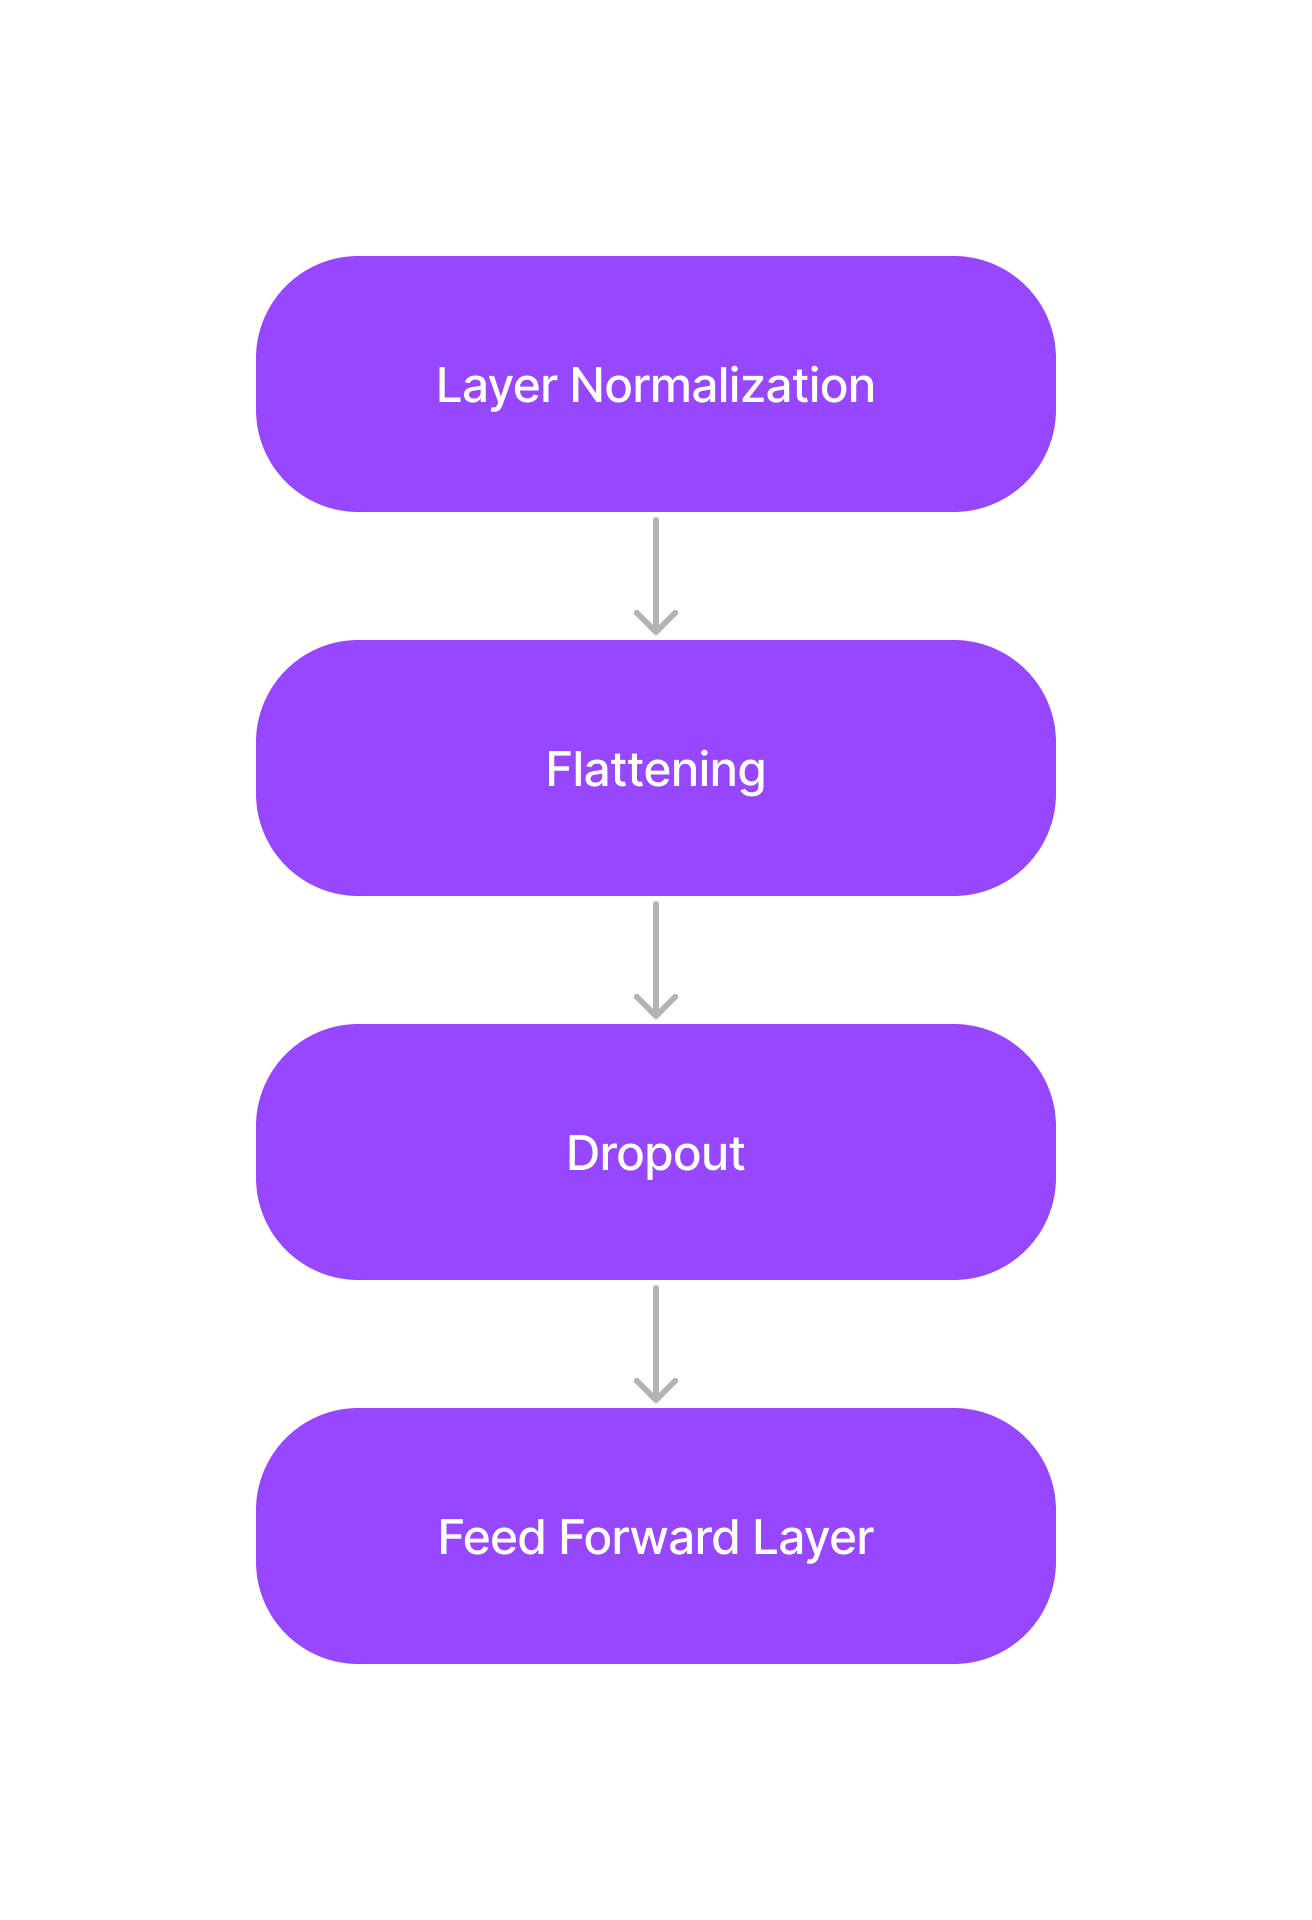
\includegraphics[width = 2in]{Ch03/representational_layer.png}
    \caption{Representational Layer}
    \label{figure:8}
\end{figure}
\begin{figure}[h]
    \centering
    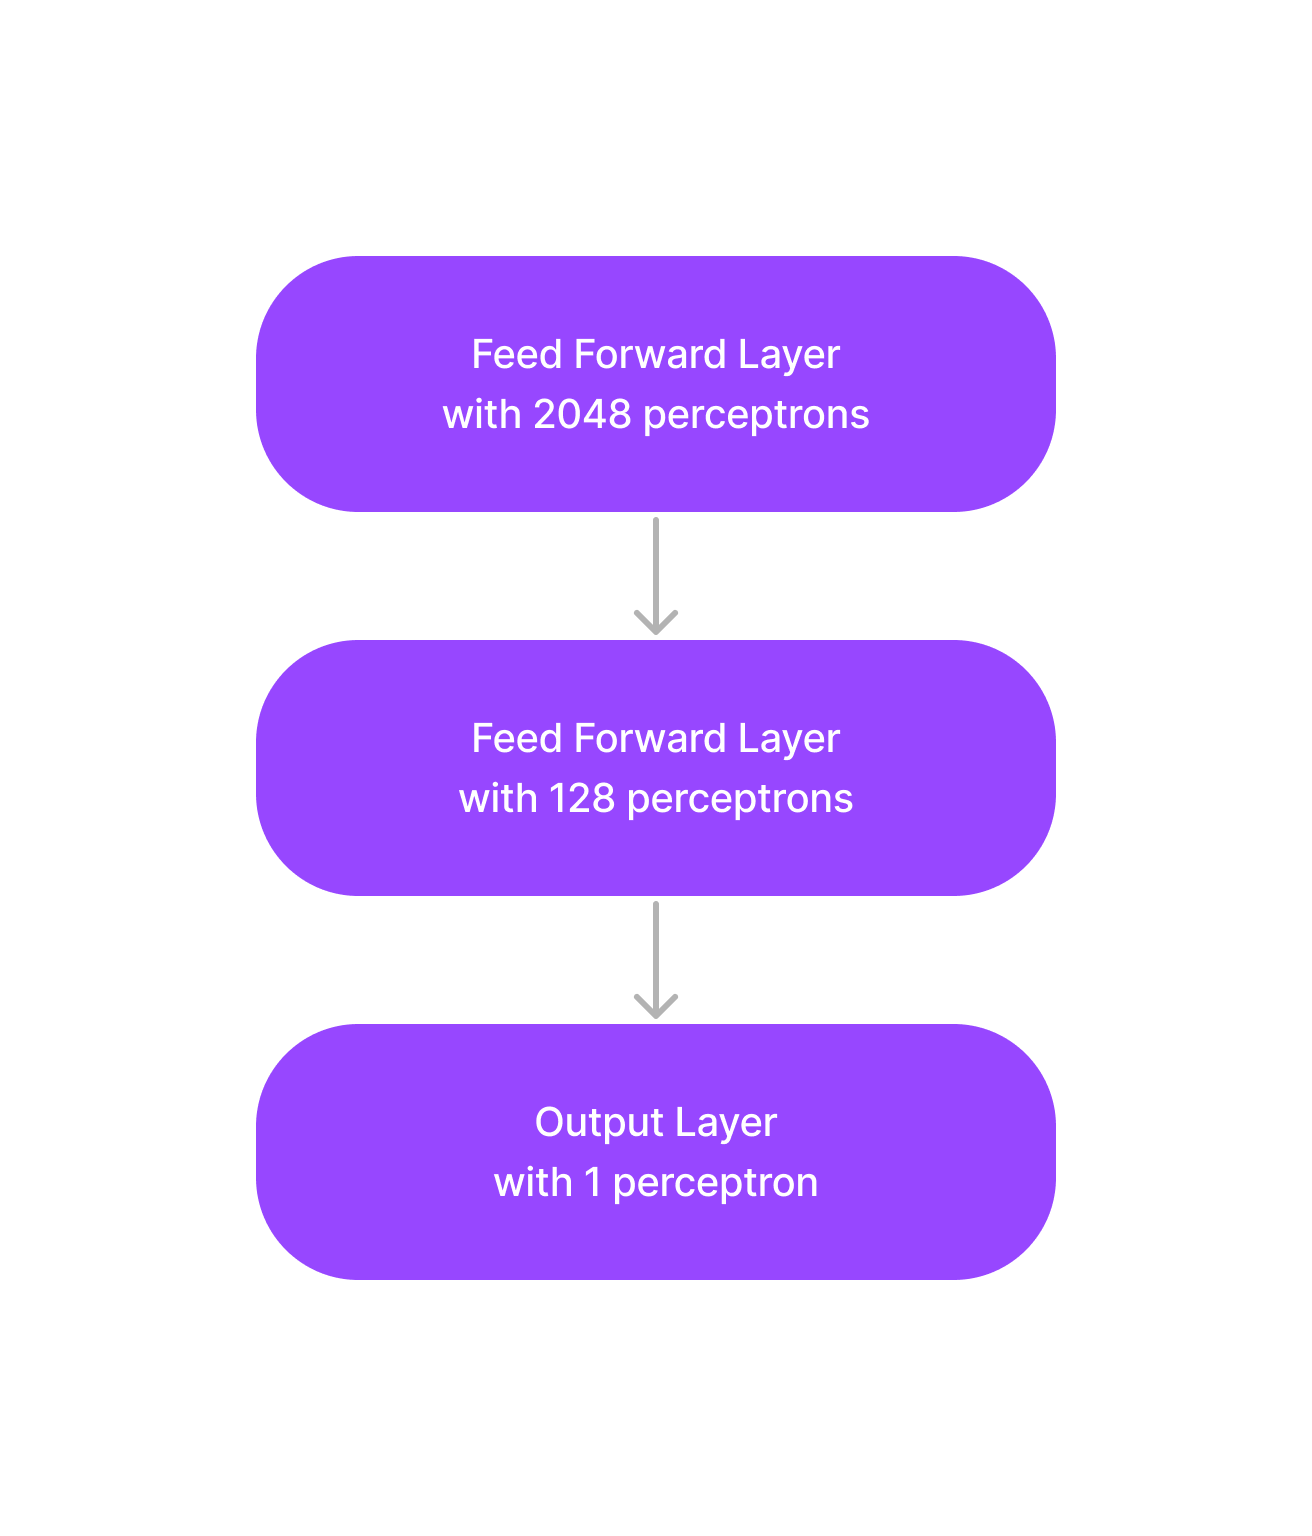
\includegraphics[width = 2in]{Ch03/classification_layer.png}
    \caption{Classification Layer}
    \label{figure:9}
\end{figure}
\FloatBarrier

\subsection{Final Model}
The main DRAN neural network is made with two input images one of the game camera recording, and other of the map processed in section 3.2.1.
\\
There are 4 output labels of the neural network namely, Throttle Value, Throttle Flag, Steering Value, Steering Flag.
\\
The final model designed is shown in figure 3.7 below.
\begin{figure}[h]
    \centering
    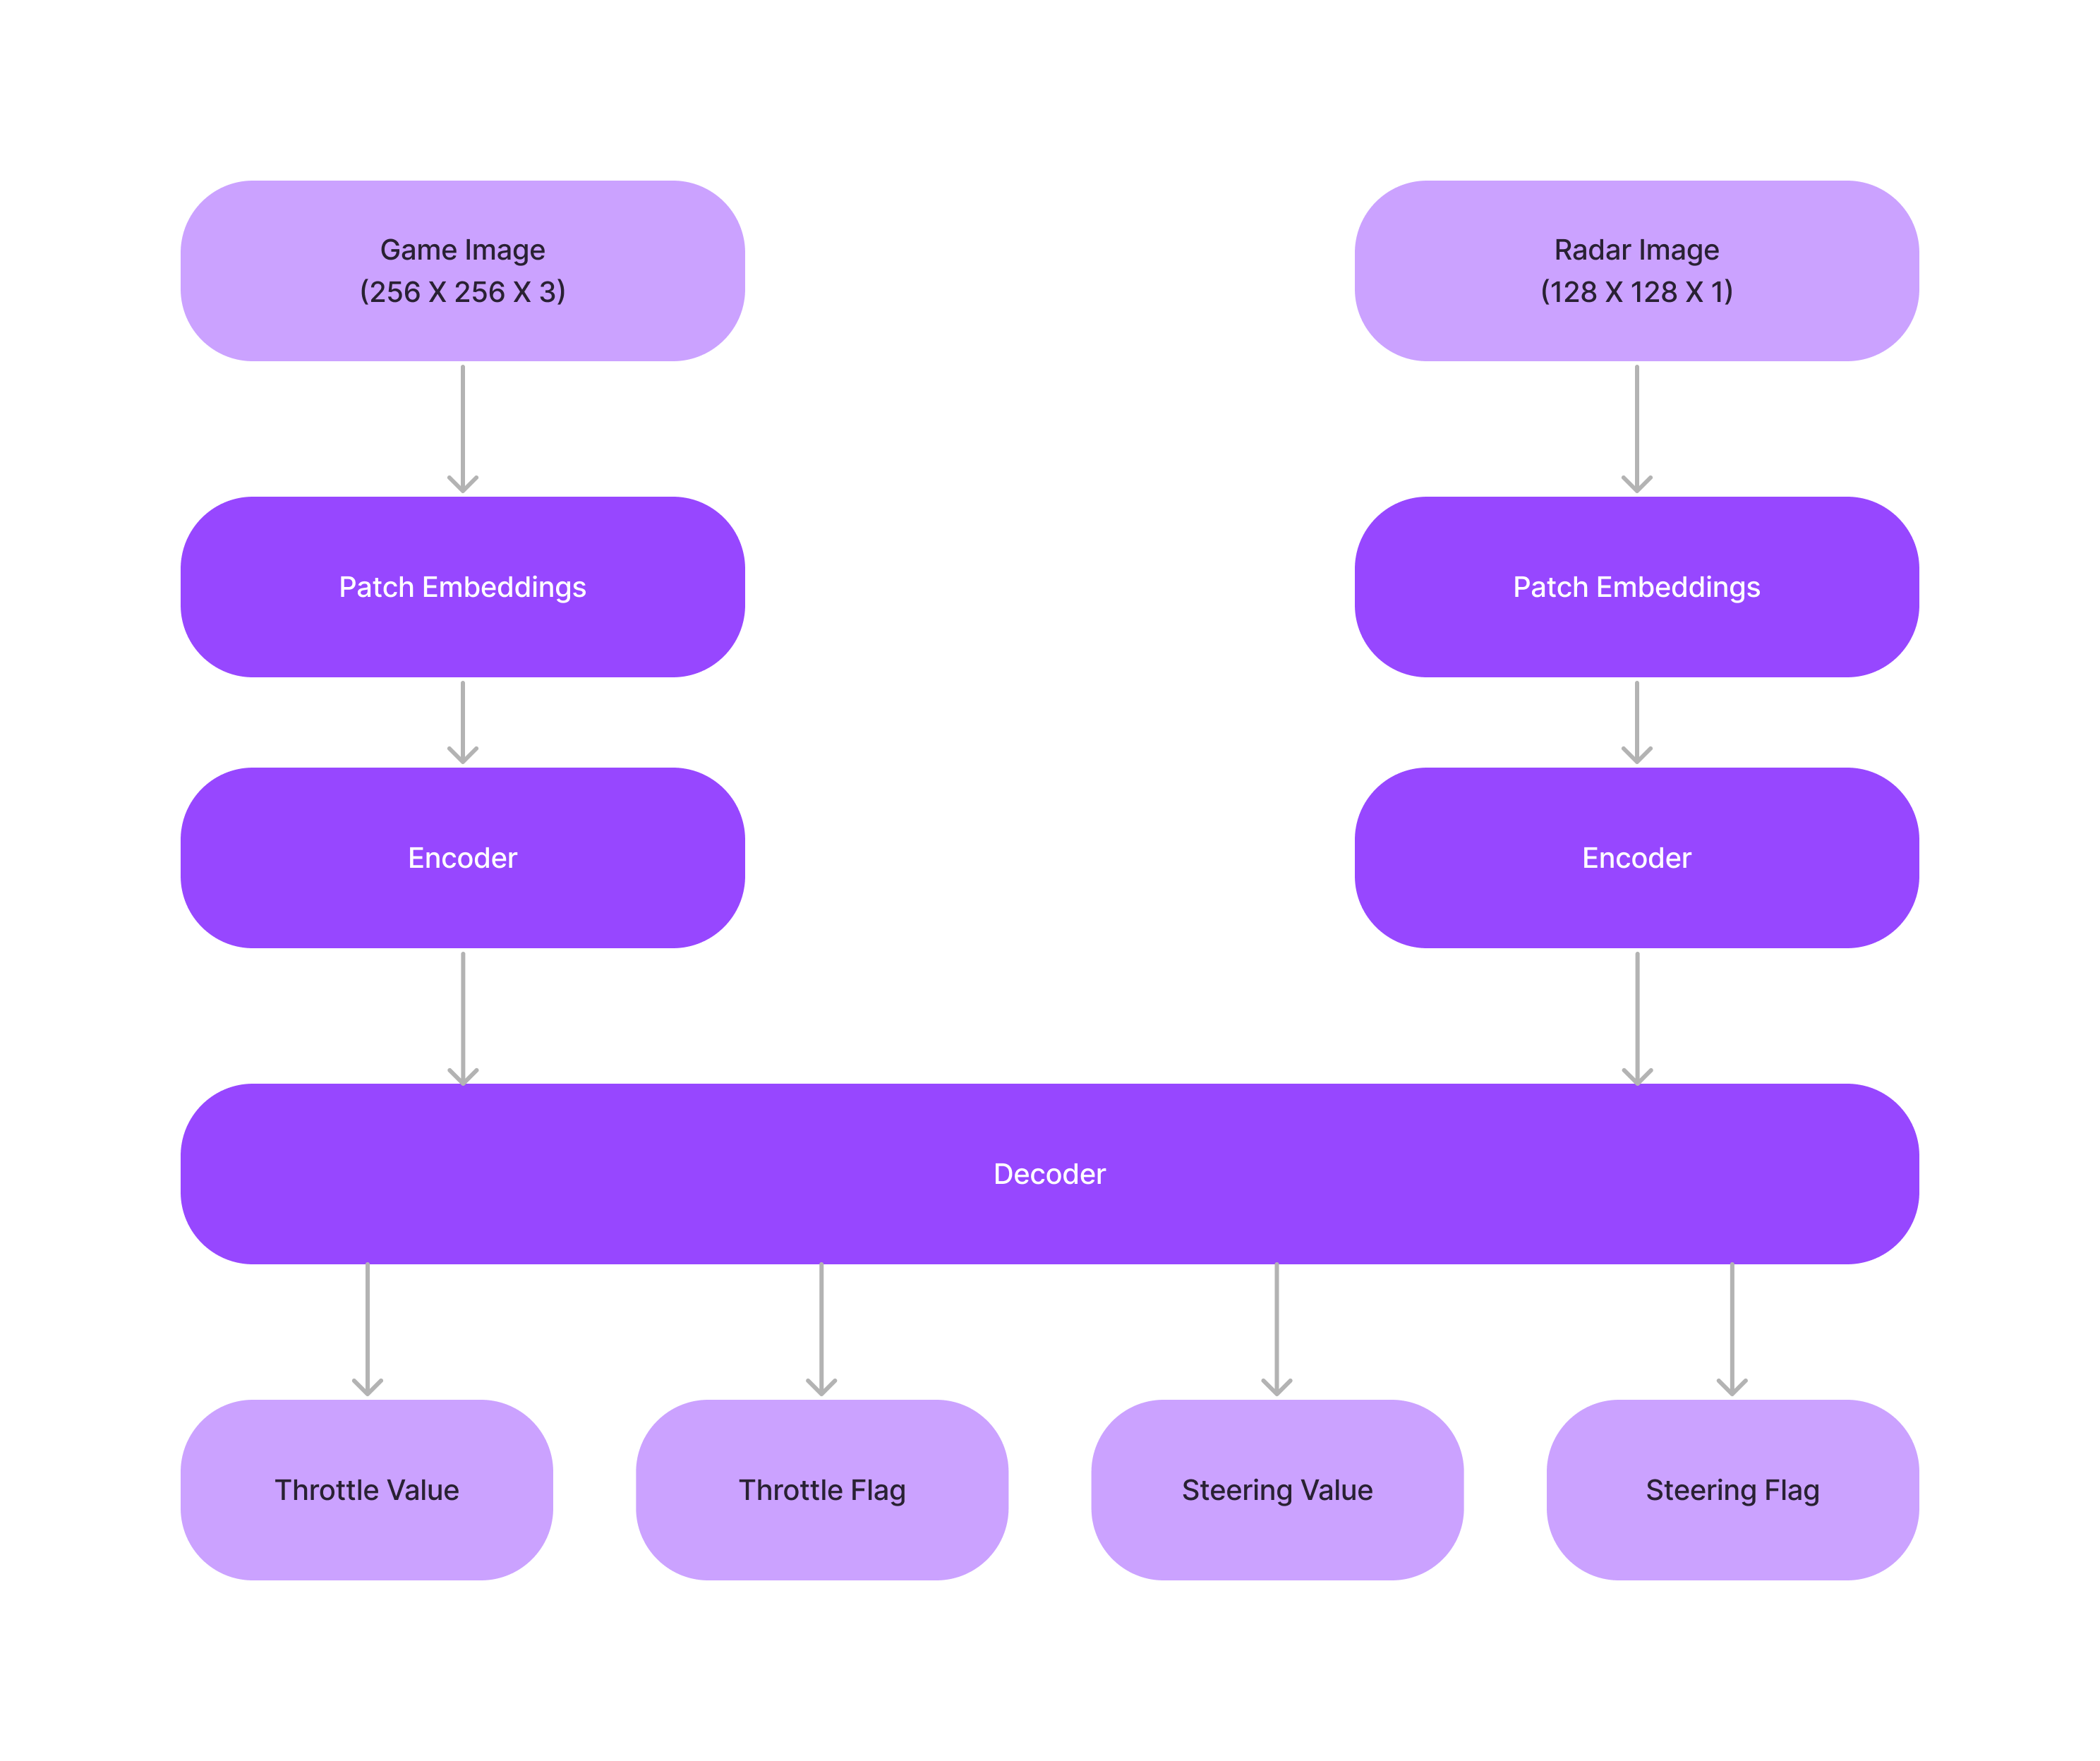
\includegraphics[width = 5in]{Ch03/dran_nn.png}
    \caption{DRAN Neural Network}
    \label{figure:10}
\end{figure}

\section{Model Preparation}
Using the above model design, a model has to be built and compiled. The model will be built in TensorFlow 2 using Keras API.

\subsection{Model Building}
The model is build considering the following hyperparameters:
\begin{itemize}
    \item Number of Encoder Layers = 6
    \item Number of Heads in Multi-Head Attention Layer = 4
    \item Number of Patches = 64
\end{itemize}
Using the following hyperparameters, the model was build and saves as dranNN.h5

\subsection{Model Compiling}
Before training, the model has to be compiled. The following specifications were used to compile the model:
\begin{itemize}
    \item Losses :  Binary Crossentropy
    \item Optimizers: Adam
    \item Metrics:
    \begin{itemize}
        \item Accuracy
        \item Mean Squared Error
      \end{itemize}
\end{itemize}

\subsection{Model Callbacks}
To assure proper training and visualization of trained model, the following callbacks are used:
\begin{itemize}
    \item Model Checkpoint
    \item Tensorboard
\end{itemize}

\subsection{Dataset Configuration}
To train the model for the first time, dataset with 10K data will be used and the datset will be splitted between train and validate in a ration of 4:1.